\documentclass[a4paper]{extarticle}

% \usepackage[T1]{fontenc}
\usepackage[utf8]{inputenc}
\usepackage[english]{babel}
\usepackage{natbib}

\usepackage{geometry}

\usepackage{subcaption}
\usepackage[mathcal]{euscript}

\usepackage{graphicx, url}

\usepackage{amsmath, amsfonts, amssymb, amsthm}
\usepackage{mathptmx}

\usepackage{grffile}

\graphicspath{{../assets/appendix/}}

\title{Bayesian Sparsification of Deep $\cplx$-valued networks -- Extended appendix}
\author{Ivan Nazarov, and Evgeny Burnaev}

%% notation
\newcommand{\real}{\mathbb{R}}
\newcommand{\cplx}{\mathbb{C}}
\newcommand{\tr}[1]{\mathop{tr}{#1}}

\newcommand{\hop}{{\mkern-1.5mu\dagger}}
\newcommand{\conj}[1]{\overline{#1}}

% \renewcommand{\top}{{\mkern-1.5mu\intercal}}
\renewcommand{\vec}[1]{\overrightarrow{#1}}
\newcommand{\diag}[1]{\mathrm{diag}{#1}}

\begin{document}
\maketitle
\tableofcontents
\listoffigures
\clearpage

\section{MNIST-like experiments} % (fold)
\label{sec:mnist_like_experiments}

The following scatter plots depict the samples from the compression-performance trade off
curve of simple networks studied in the experiments on the MNIST-like datasets. Transparent
horizontal bands on each plot represent min-max performance spread of an uncompressed
network on the test split. The points illustrate the final trade-off of the compressed
networks after fine-tuning, while their tails show the performance gain or loss due to
the fine-tuning.

We recap the set up of each experiment on MNIST-like:
\begin{itemize}
  \item staged training, with weight and optimizer state transfer
  \item $40$, $75$, and $40$ epochs for ``dense'', ``sparsify'', and ``fine-tune'' stagers, respectively
  \item ADAM optimizer with learning rate $10^{-3}$ before the $10$-th, and $10^{-4}$
  afterwards
  \item $\ell_2$-norm global gradient clipping at $\tfrac12$
  \item training batches of size $128$ from a fixed randomly subset ($10^4$ images) of the training split
  \item the multiplier of the Kullback-Leibler term in ELBO varies over $
    C \in \{
      \tfrac32 2^{-\tfrac{k}2} \colon k=2, \cdots, 38
    \}
  $
  \item the sparsification threshold $\tau$ is set to $-\tfrac12$
\end{itemize}
Each experiment was performed $5$ times to obtain a small sample of performance-compression
values for each setting of $C$. By reevaluating each setting several times we can account
for randomness in initialization of the uncompressed network at ``dense'', stochasticity of
variational dropout layers, and randomness of batch sequences during SDG, and non-determinism
of computations on GPUs.

Each figure shows the compression-accuracy trade-off of a particular method and input features
for \textit{SimpleConvModel} and \textit{TwoLayerDenseModel} models for all four of the studied
datasets (described in the main text): \emph{top-left} EMNIST-Letters, \emph{top-right} KMNIST,
\emph{bottom-left} Fashion MNIST, and \emph{bottom-right} MNIST.
%
Figures \ref{fig:appendix__mnist-like__trade-off__ARD__fft}, \ref{fig:appendix__mnist-like__trade-off__VD__fft},
\ref{fig:appendix__mnist-like__trade-off__ARD__raw}, and \ref{fig:appendix__mnist-like__trade-off__VD__raw}
compare $\real$ models against $\cplx$ with \emph{the same architecture}, i.e. incomparable
according to \citet{monning_evaluation_2018}. We also report the trade-off comparison, when
their argument for higher intrinsic capacity of $\cplx$-valued networks has been taken
into account.
%
We compare $\real$ networks against $\tfrac12 \cplx$ with half the number of parameters
for raw input features on figures \ref{fig:appendix__cmp__mnist-like__trade-off__ARD__raw},
and \ref{fig:appendix__cmp__mnist-like__trade-off__VD__raw}, and $2 \real$ with
double the number of parameters against $\cplx$ for Fourier input features on figures
\ref{fig:appendix__cmp__mnist-like__trade-off__ARD__fft} and
\ref{fig:appendix__cmp__mnist-like__trade-off__VD__fft}.

The following observations could be made from the conducted experiment:
\begin{itemize}
  \item $\cplx$-valued networks do not have as much spare capacity as $2 \real$ due to
  constants imposed by multiplication in $\cplx$ numbers (\ref{fig:appendix__cmp__mnist-like__trade-off__ARD__raw},
  \ref{fig:appendix__cmp__mnist-like__trade-off__VD__raw})
  \item Variational Dropout and Automatic Relevance Determination offer similar compression-performance
  trade-off, with negligibly lower compression by the latter (both $\real$ and $\cplx$ versions,
  e.g. figures \ref{fig:appendix__mnist-like__trade-off__ARD__raw} and \ref{fig:appendix__mnist-like__trade-off__VD__raw})
  \item smaller networks tend to be less compressible (figures \ref{fig:appendix__cmp__mnist-like__trade-off__ARD__fft},
  \ref{fig:appendix__cmp__mnist-like__trade-off__VD__fft})
\end{itemize}

\begin{figure}[ht]
  \centering
  \begin{subfigure}[b]{0.5\textwidth}
    \centering
    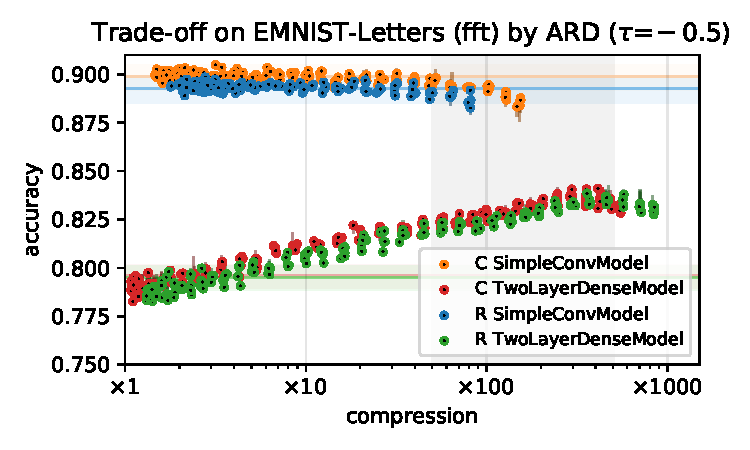
\includegraphics[width=\linewidth]{figure__mnist-like__trade-off/appendix__ARD__emnist_letters__fft__-0.5.pdf}
  \end{subfigure}%
  \begin{subfigure}[b]{0.5\textwidth}
    \centering
    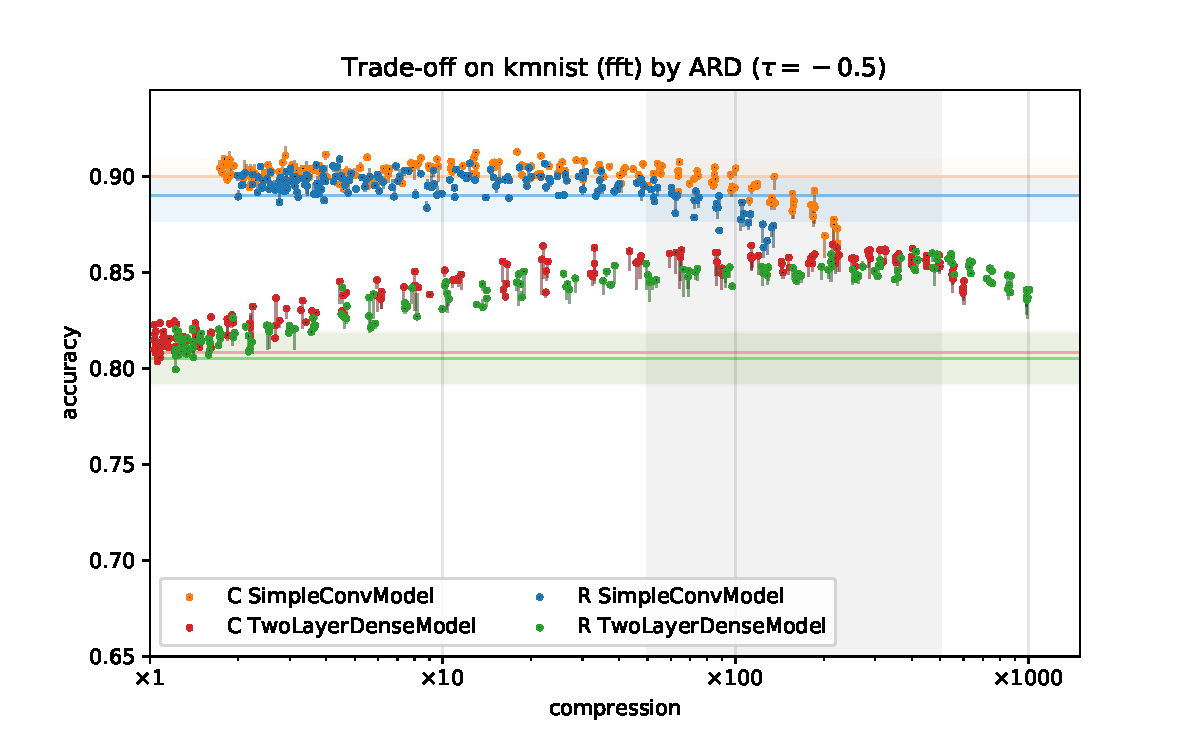
\includegraphics[width=\linewidth]{figure__mnist-like__trade-off/appendix__ARD__kmnist__fft__-0.5.pdf}
  \end{subfigure} \\ %
  \begin{subfigure}[b]{0.5\textwidth}
    \centering
    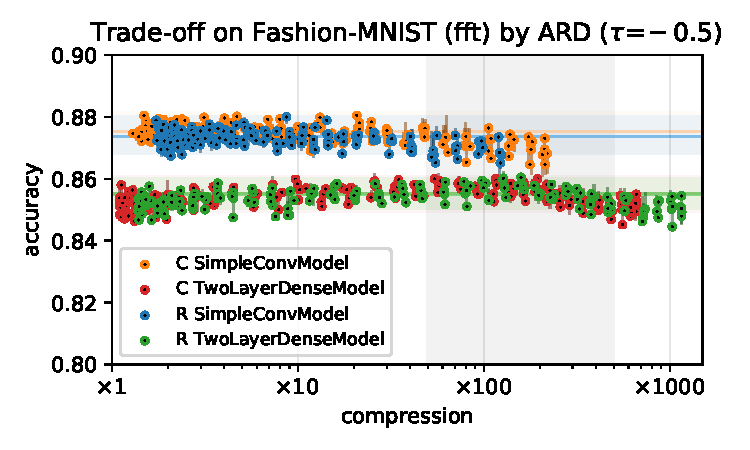
\includegraphics[width=\linewidth]{figure__mnist-like__trade-off/appendix__ARD__fashionmnist__fft__-0.5.pdf}
  \end{subfigure}%
  \begin{subfigure}[b]{0.5\textwidth}
    \centering
    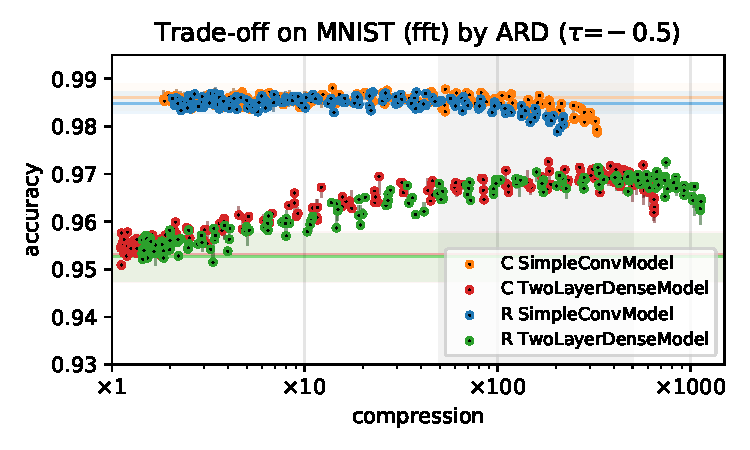
\includegraphics[width=\linewidth]{figure__mnist-like__trade-off/appendix__ARD__mnist__fft__-0.5.pdf}
  \end{subfigure}
  \caption{%
    The compression-accuracy trade-off of ARD method for $\real$ and $\cplx$ models using Fourier features.
  }
  \label{fig:appendix__mnist-like__trade-off__ARD__fft}
\end{figure}

\begin{figure}[ht]
  \centering
  \begin{subfigure}[b]{0.5\textwidth}
    \centering
    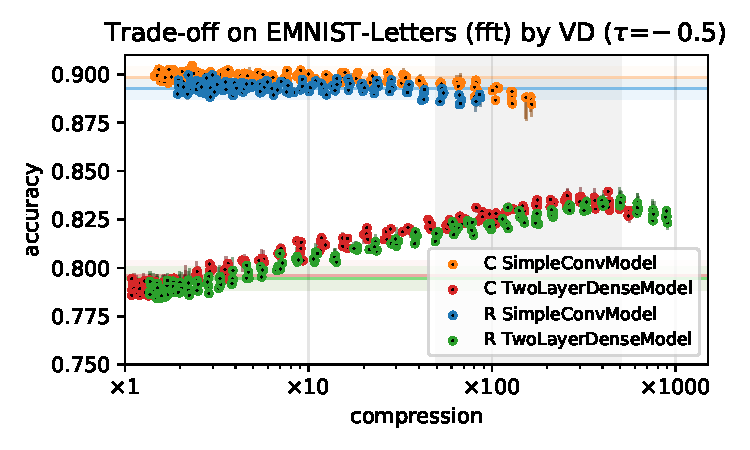
\includegraphics[width=\linewidth]{figure__mnist-like__trade-off/appendix__VD__emnist_letters__fft__-0.5.pdf}
  \end{subfigure}%
  \begin{subfigure}[b]{0.5\textwidth}
    \centering
    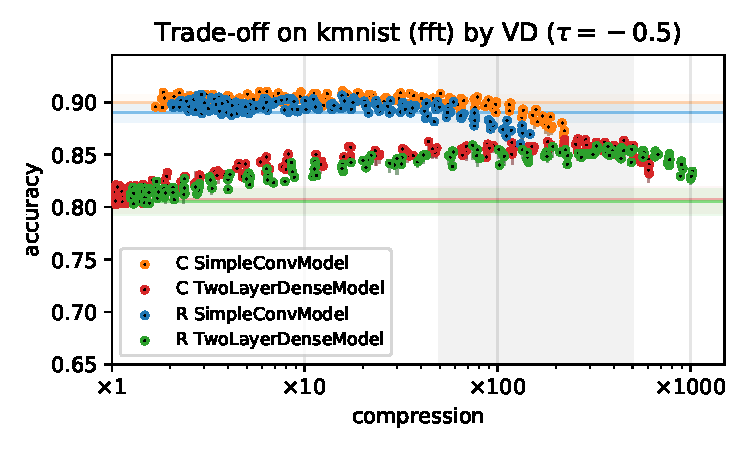
\includegraphics[width=\linewidth]{figure__mnist-like__trade-off/appendix__VD__kmnist__fft__-0.5.pdf}
  \end{subfigure} \\ %
  \begin{subfigure}[b]{0.5\textwidth}
    \centering
    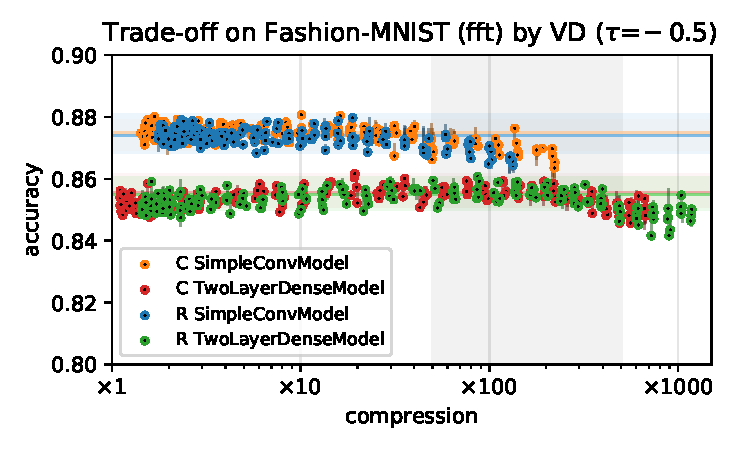
\includegraphics[width=\linewidth]{figure__mnist-like__trade-off/appendix__VD__fashionmnist__fft__-0.5.pdf}
  \end{subfigure}%
  \begin{subfigure}[b]{0.5\textwidth}
    \centering
    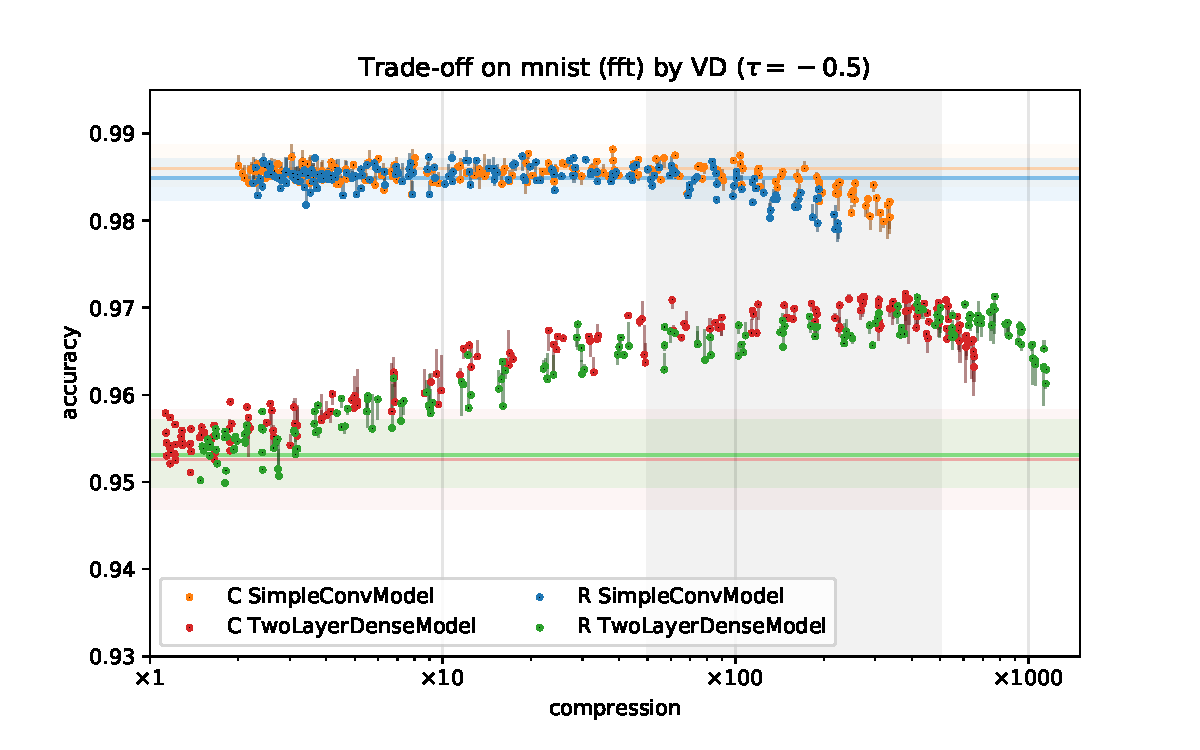
\includegraphics[width=\linewidth]{figure__mnist-like__trade-off/appendix__VD__mnist__fft__-0.5.pdf}
  \end{subfigure}
  \caption{%
    The compression-accuracy trade-off of VD method for $\real$ and $\cplx$ models using Fourier features.
  }
  \label{fig:appendix__mnist-like__trade-off__VD__fft}
\end{figure}

\begin{figure}[ht]
  \centering
  \begin{subfigure}[b]{0.5\textwidth}
    \centering
    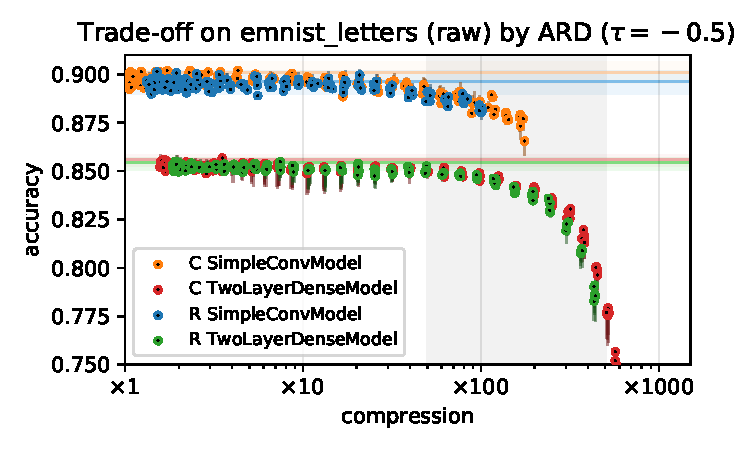
\includegraphics[width=\linewidth]{figure__mnist-like__trade-off/appendix__ARD__emnist_letters__raw__-0.5.pdf}
  \end{subfigure}%
  \begin{subfigure}[b]{0.5\textwidth}
    \centering
    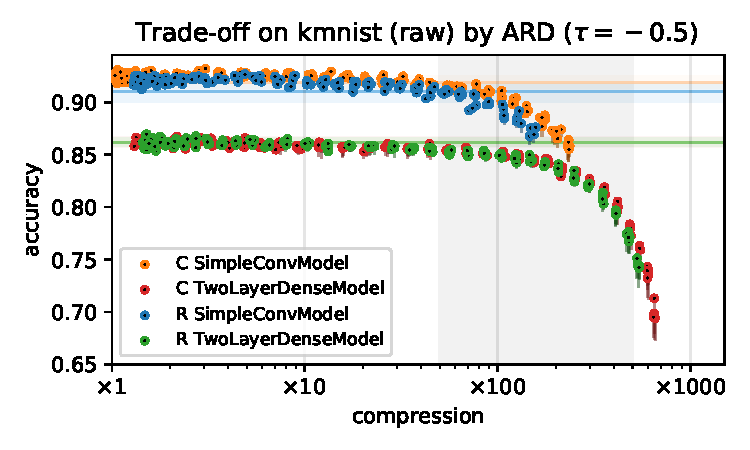
\includegraphics[width=\linewidth]{figure__mnist-like__trade-off/appendix__ARD__kmnist__raw__-0.5.pdf}
  \end{subfigure} \\%
  \begin{subfigure}[b]{0.5\textwidth}
    \centering
    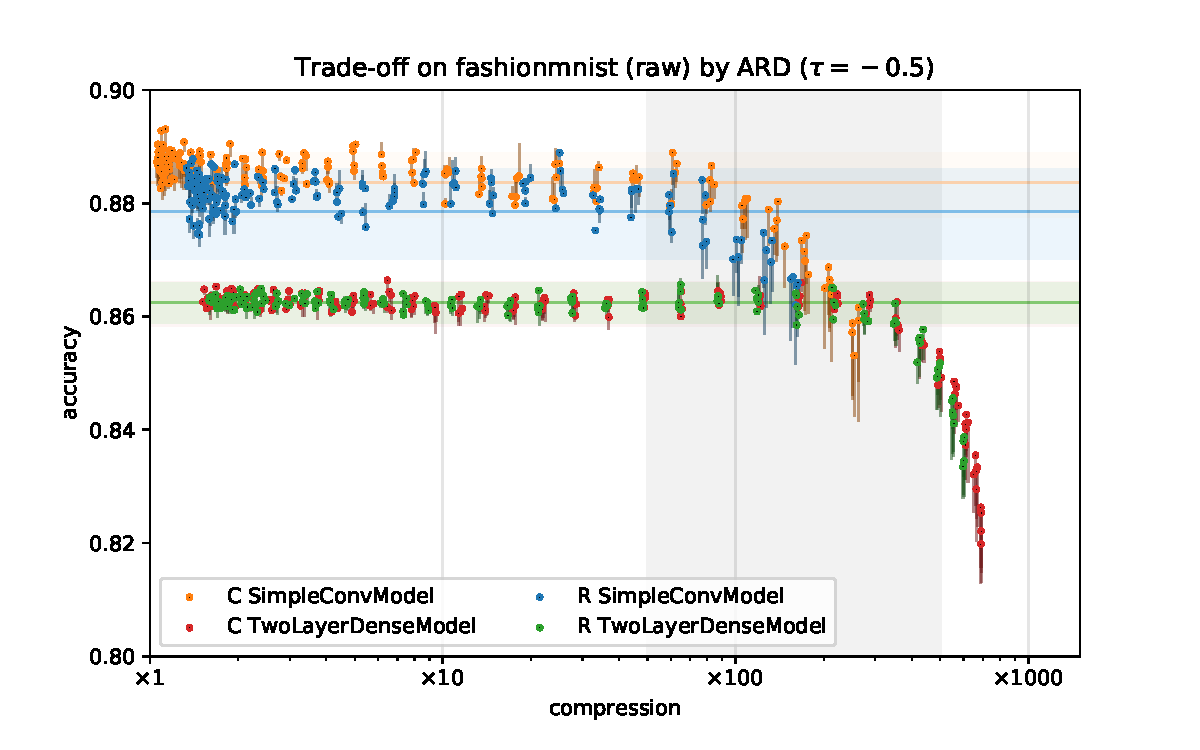
\includegraphics[width=\linewidth]{figure__mnist-like__trade-off/appendix__ARD__fashionmnist__raw__-0.5.pdf}
  \end{subfigure}%
  \begin{subfigure}[b]{0.5\textwidth}
    \centering
    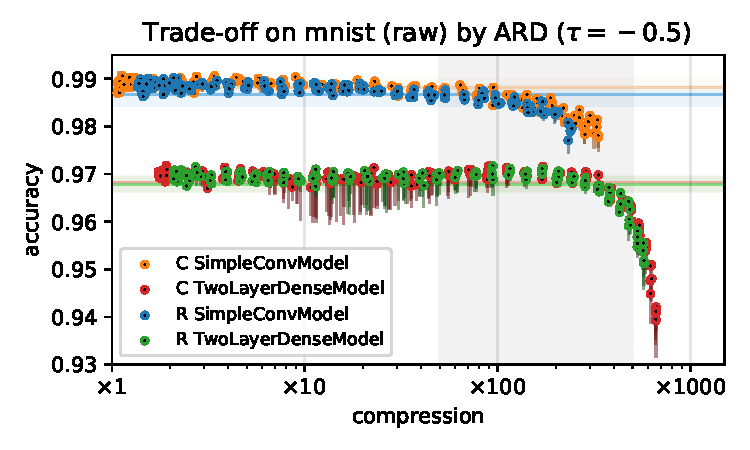
\includegraphics[width=\linewidth]{figure__mnist-like__trade-off/appendix__ARD__mnist__raw__-0.5.pdf}
  \end{subfigure}
  \caption{%
    The compression-accuracy trade-off of ARD method for $\real$ and $\cplx$ models using raw features.
  }
  \label{fig:appendix__mnist-like__trade-off__ARD__raw}
\end{figure}

\begin{figure}[ht]
  \centering
  \begin{subfigure}[b]{0.5\textwidth}
    \centering
    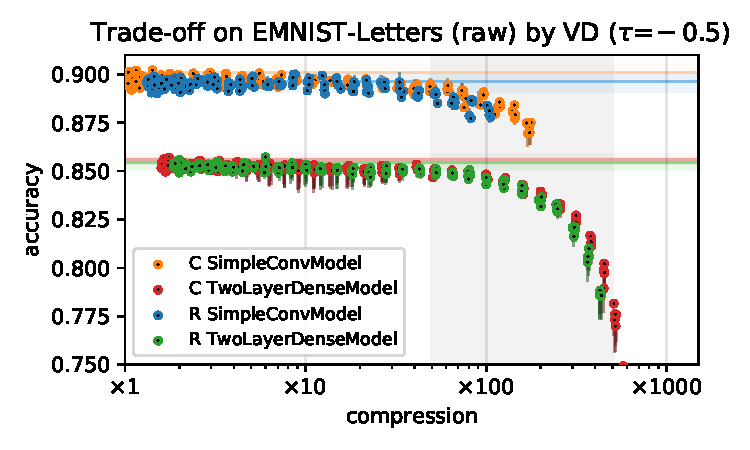
\includegraphics[width=\linewidth]{figure__mnist-like__trade-off/appendix__VD__emnist_letters__raw__-0.5.pdf}
  \end{subfigure}%
  \begin{subfigure}[b]{0.5\textwidth}
    \centering
    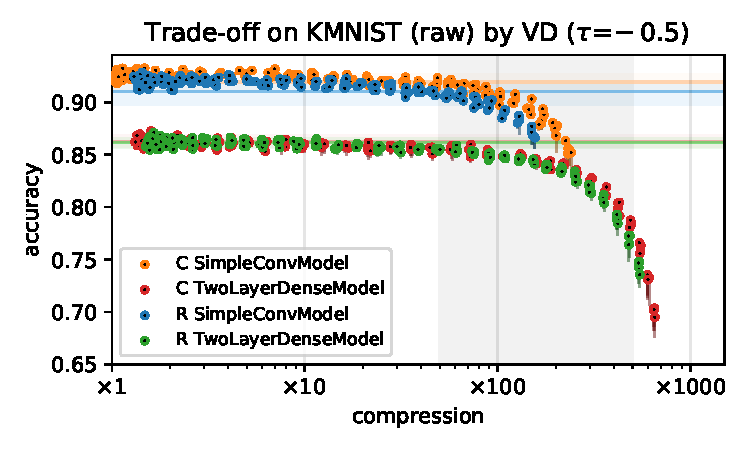
\includegraphics[width=\linewidth]{figure__mnist-like__trade-off/appendix__VD__kmnist__raw__-0.5.pdf}
  \end{subfigure} \\%
  \begin{subfigure}[b]{0.5\textwidth}
    \centering
    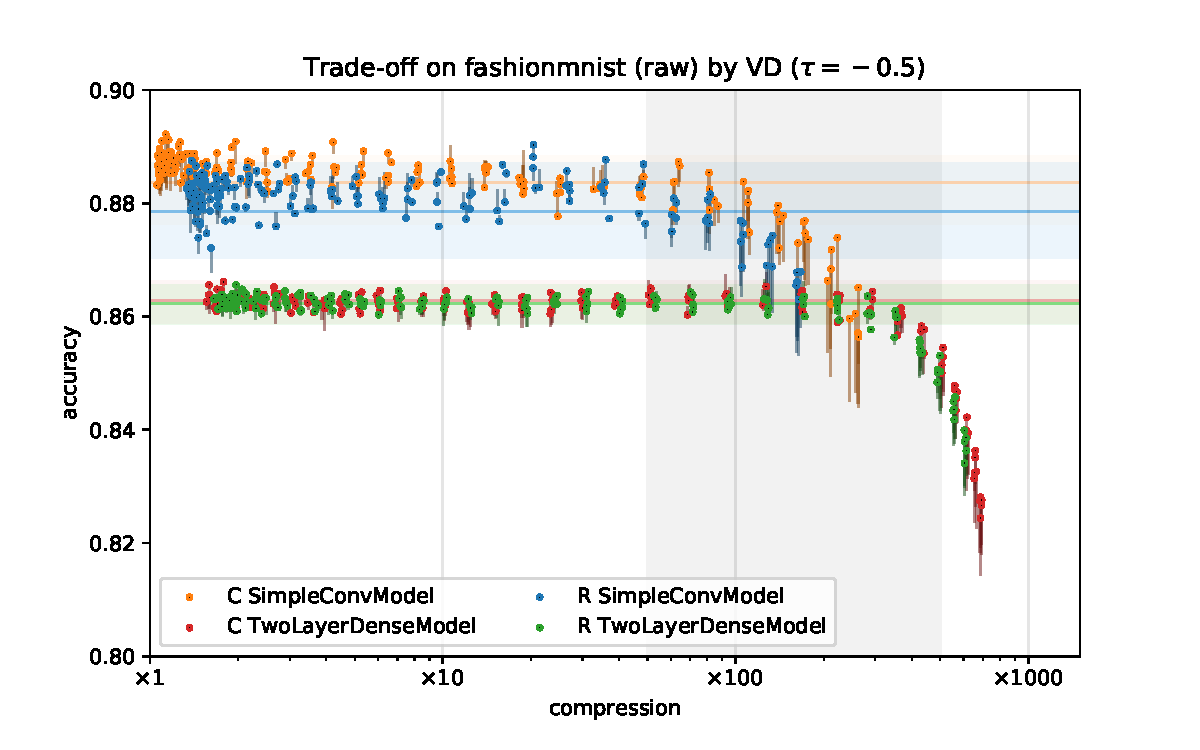
\includegraphics[width=\linewidth]{figure__mnist-like__trade-off/appendix__VD__fashionmnist__raw__-0.5.pdf}
  \end{subfigure}%
  \begin{subfigure}[b]{0.5\textwidth}
    \centering
    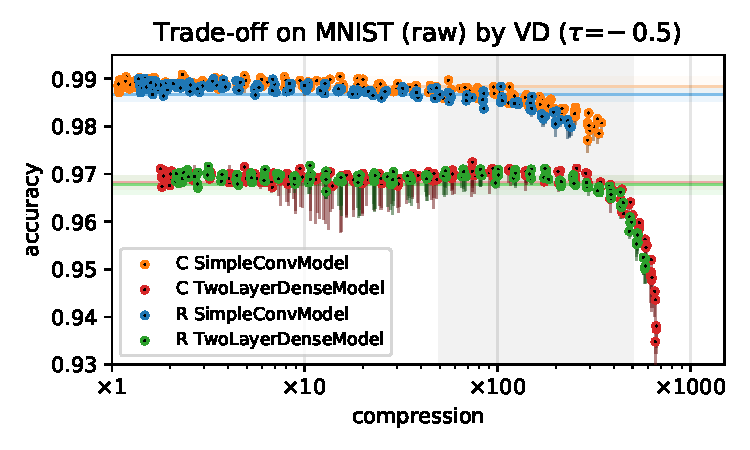
\includegraphics[width=\linewidth]{figure__mnist-like__trade-off/appendix__VD__mnist__raw__-0.5.pdf}
  \end{subfigure}
  \caption{%
    The compression-accuracy trade-off of VD method for $\real$ and $\cplx$ models using raw features.
  }
  \label{fig:appendix__mnist-like__trade-off__VD__raw}
\end{figure}

\begin{figure}[ht]
  \centering
  \begin{subfigure}[b]{0.5\textwidth}
    \centering
    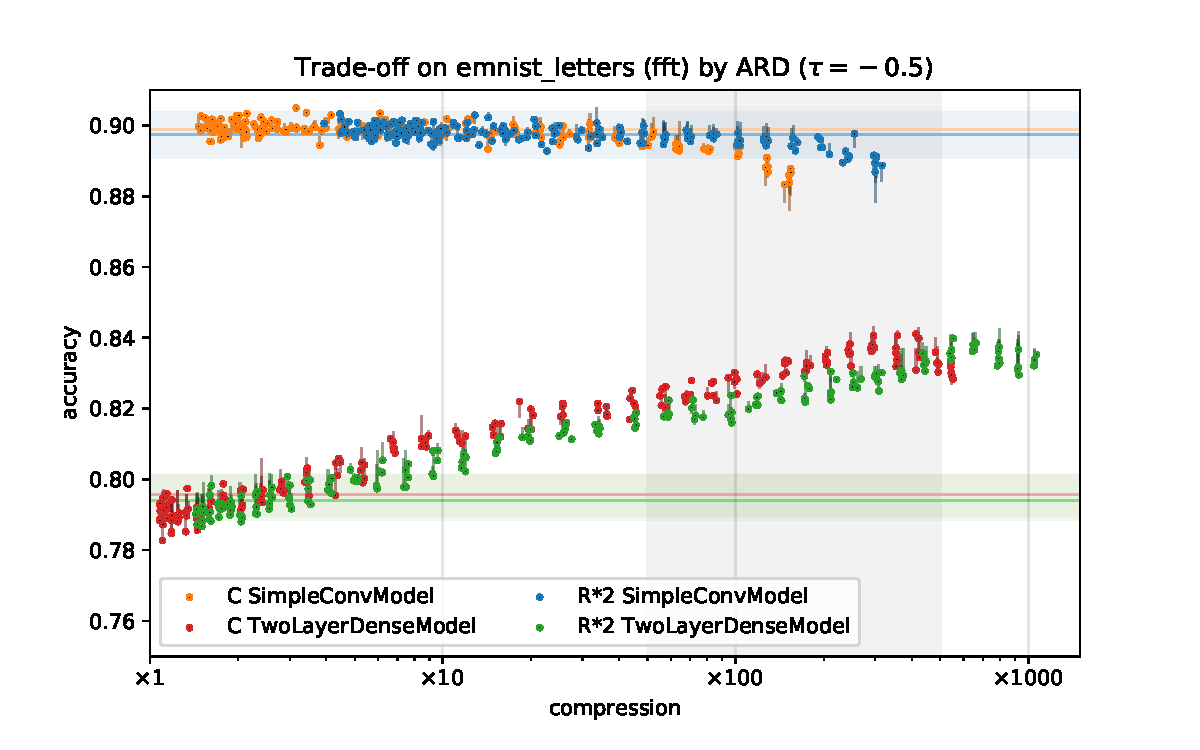
\includegraphics[width=\linewidth]{figure__mnist-like__trade-off/appendix__cmp__ARD__emnist_letters__fft__-0.5.pdf}
  \end{subfigure}%
  \begin{subfigure}[b]{0.5\textwidth}
    \centering
    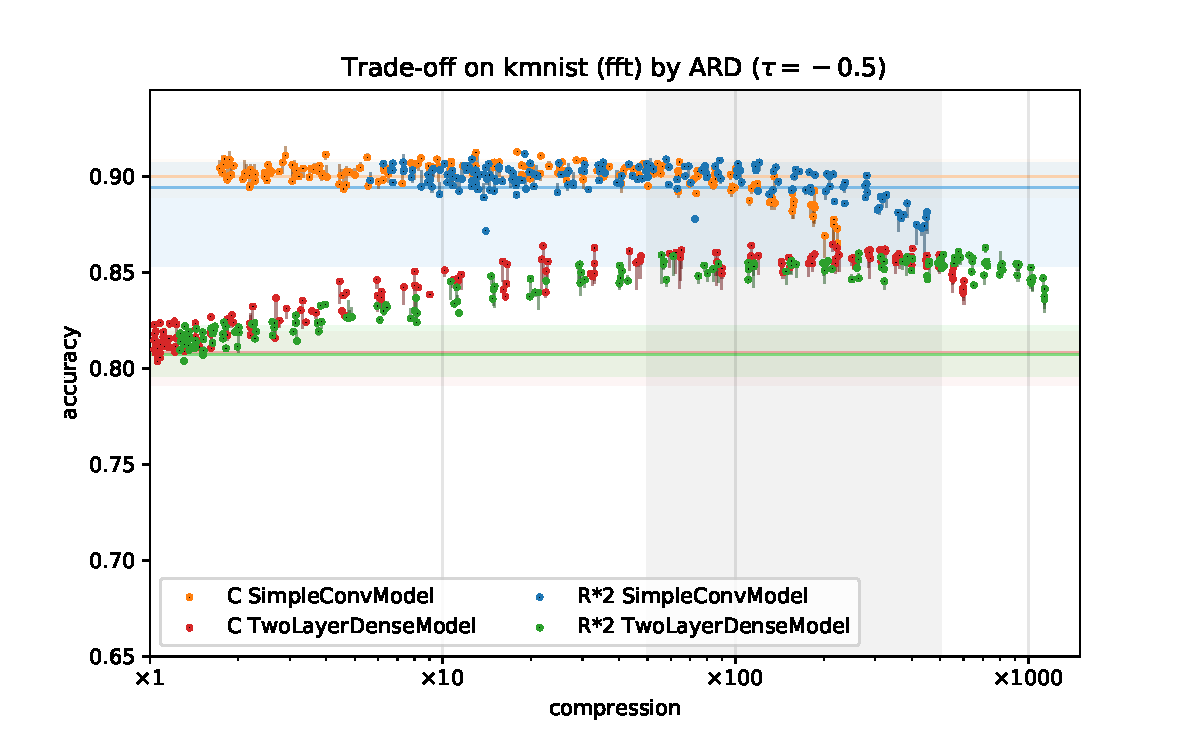
\includegraphics[width=\linewidth]{figure__mnist-like__trade-off/appendix__cmp__ARD__kmnist__fft__-0.5.pdf}
  \end{subfigure} \\ %
  \begin{subfigure}[b]{0.5\textwidth}
    \centering
    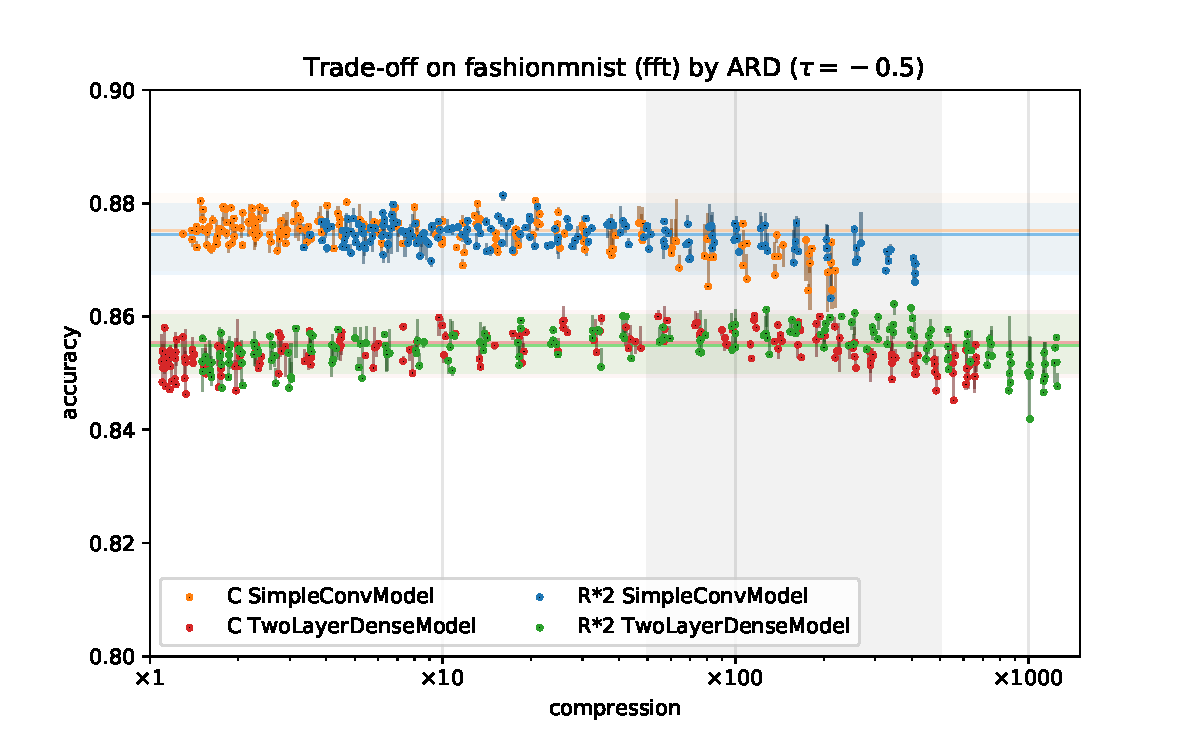
\includegraphics[width=\linewidth]{figure__mnist-like__trade-off/appendix__cmp__ARD__fashionmnist__fft__-0.5.pdf}
  \end{subfigure}%
  \begin{subfigure}[b]{0.5\textwidth}
    \centering
    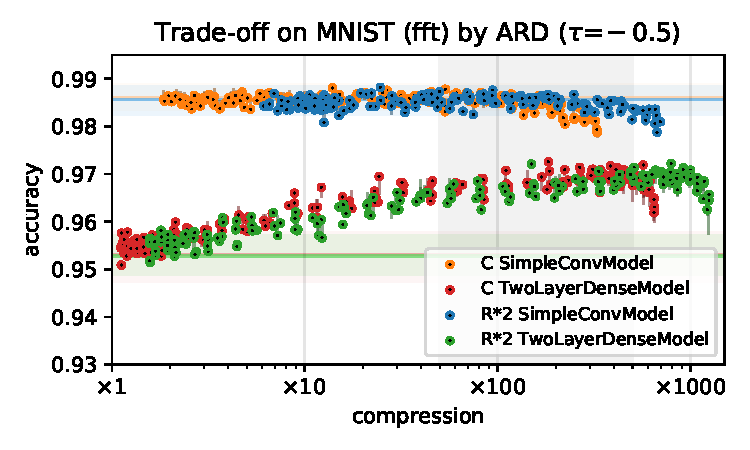
\includegraphics[width=\linewidth]{figure__mnist-like__trade-off/appendix__cmp__ARD__mnist__fft__-0.5.pdf}
  \end{subfigure}
  \caption{%
    The compression-accuracy trade-off of ARD method for $2\real$ and $\cplx$ models using Fourier features.
  }
  \label{fig:appendix__cmp__mnist-like__trade-off__ARD__fft}
\end{figure}

\begin{figure}[ht]
  \centering
  \begin{subfigure}[b]{0.5\textwidth}
    \centering
    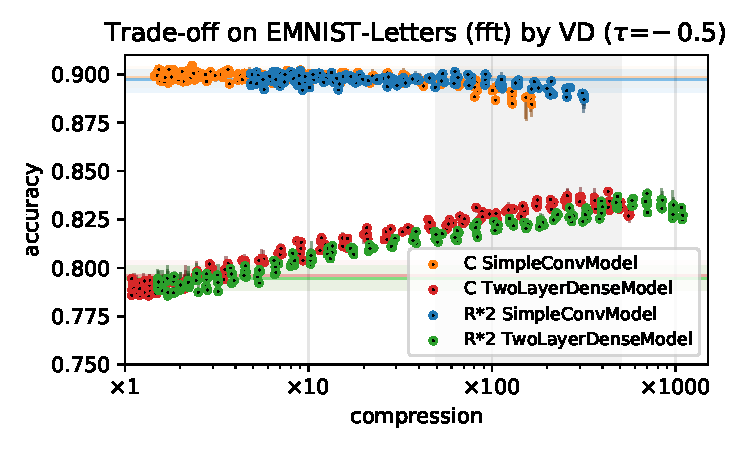
\includegraphics[width=\linewidth]{figure__mnist-like__trade-off/appendix__cmp__VD__emnist_letters__fft__-0.5.pdf}
  \end{subfigure}%
  \begin{subfigure}[b]{0.5\textwidth}
    \centering
    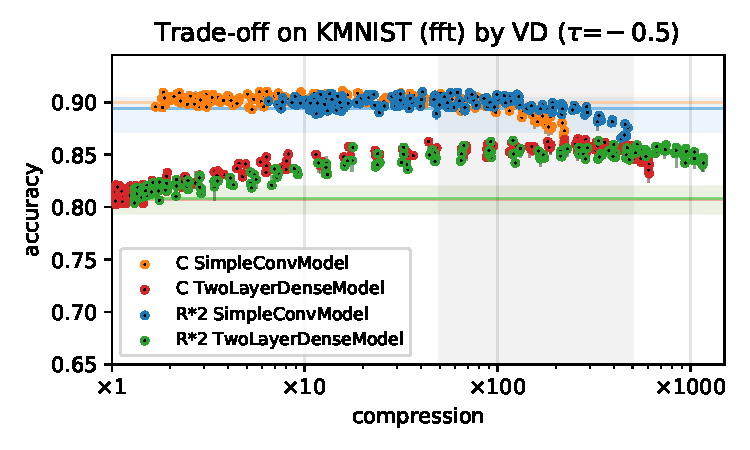
\includegraphics[width=\linewidth]{figure__mnist-like__trade-off/appendix__cmp__VD__kmnist__fft__-0.5.pdf}
  \end{subfigure} \\ %
  \begin{subfigure}[b]{0.5\textwidth}
    \centering
    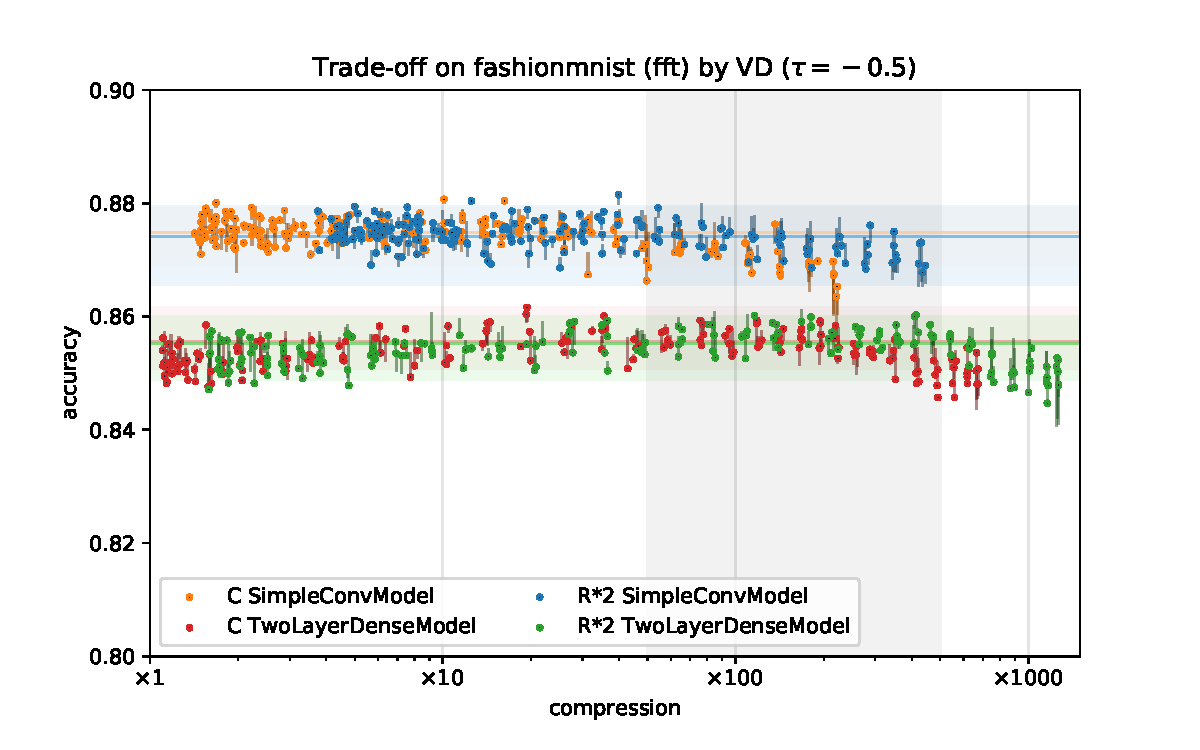
\includegraphics[width=\linewidth]{figure__mnist-like__trade-off/appendix__cmp__VD__fashionmnist__fft__-0.5.pdf}
  \end{subfigure}%
  \begin{subfigure}[b]{0.5\textwidth}
    \centering
    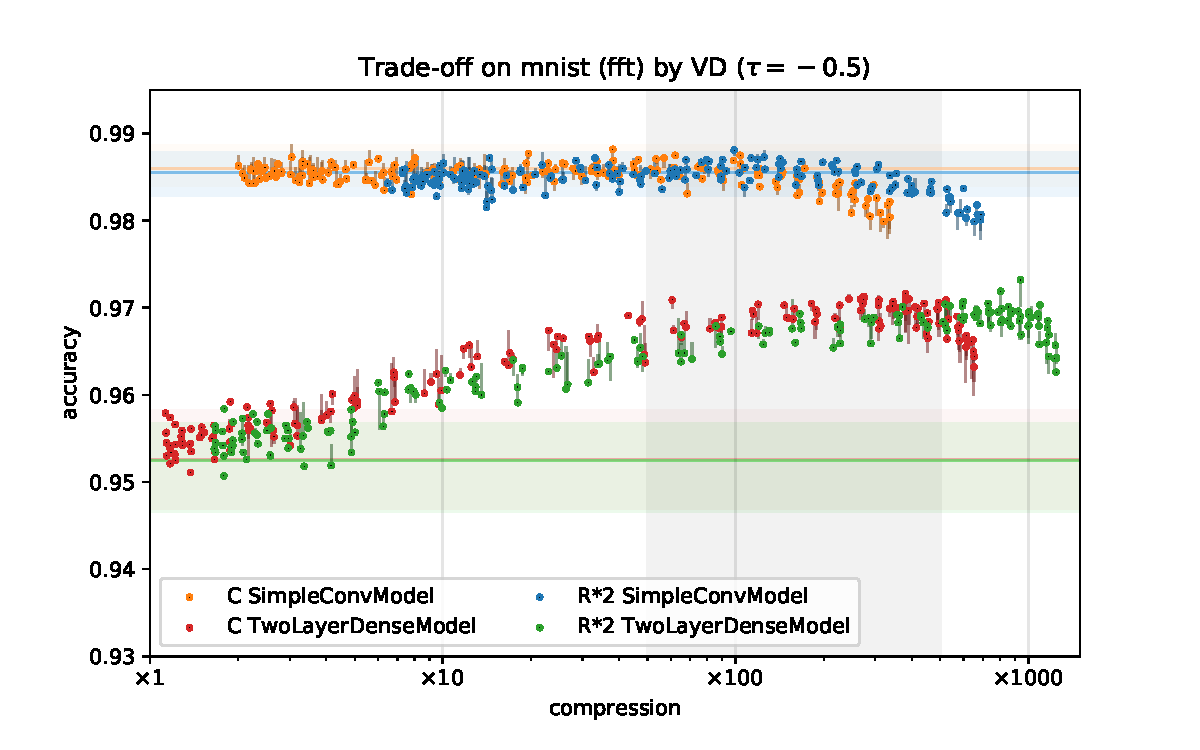
\includegraphics[width=\linewidth]{figure__mnist-like__trade-off/appendix__cmp__VD__mnist__fft__-0.5.pdf}
  \end{subfigure}
  \caption{%
    The compression-accuracy trade-off of VD method for $2\real$ and $\cplx$ models using Fourier features.
  }
  \label{fig:appendix__cmp__mnist-like__trade-off__VD__fft}
\end{figure}

\begin{figure}[ht]
  \centering
  \begin{subfigure}[b]{0.5\textwidth}
    \centering
    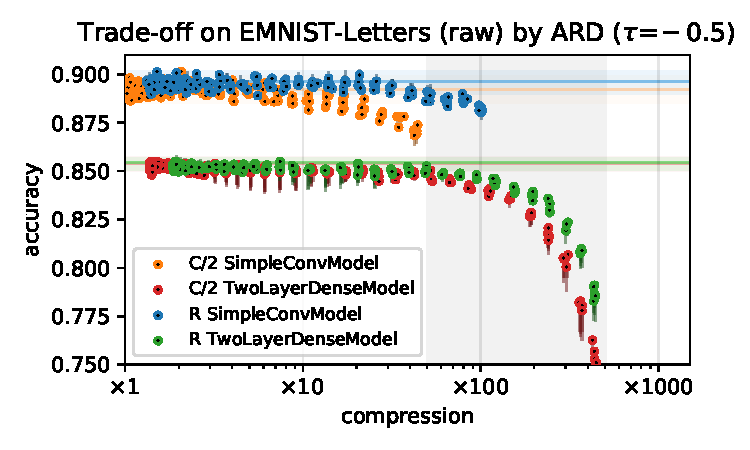
\includegraphics[width=\linewidth]{figure__mnist-like__trade-off/appendix__cmp__ARD__emnist_letters__raw__-0.5.pdf}
  \end{subfigure}%
  \begin{subfigure}[b]{0.5\textwidth}
    \centering
    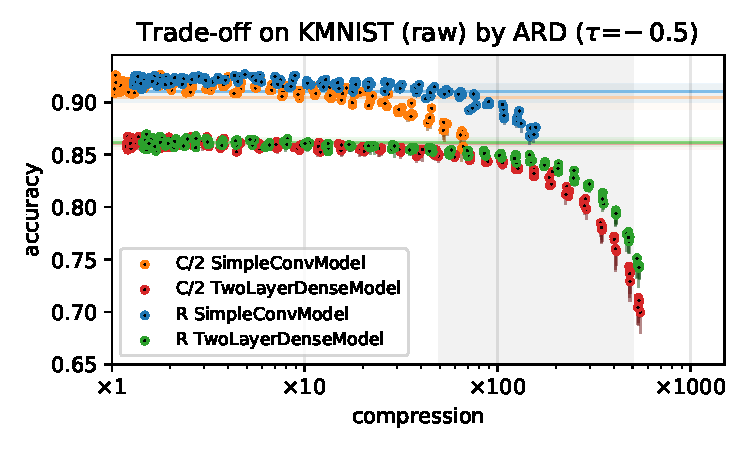
\includegraphics[width=\linewidth]{figure__mnist-like__trade-off/appendix__cmp__ARD__kmnist__raw__-0.5.pdf}
  \end{subfigure} \\%
  \begin{subfigure}[b]{0.5\textwidth}
    \centering
    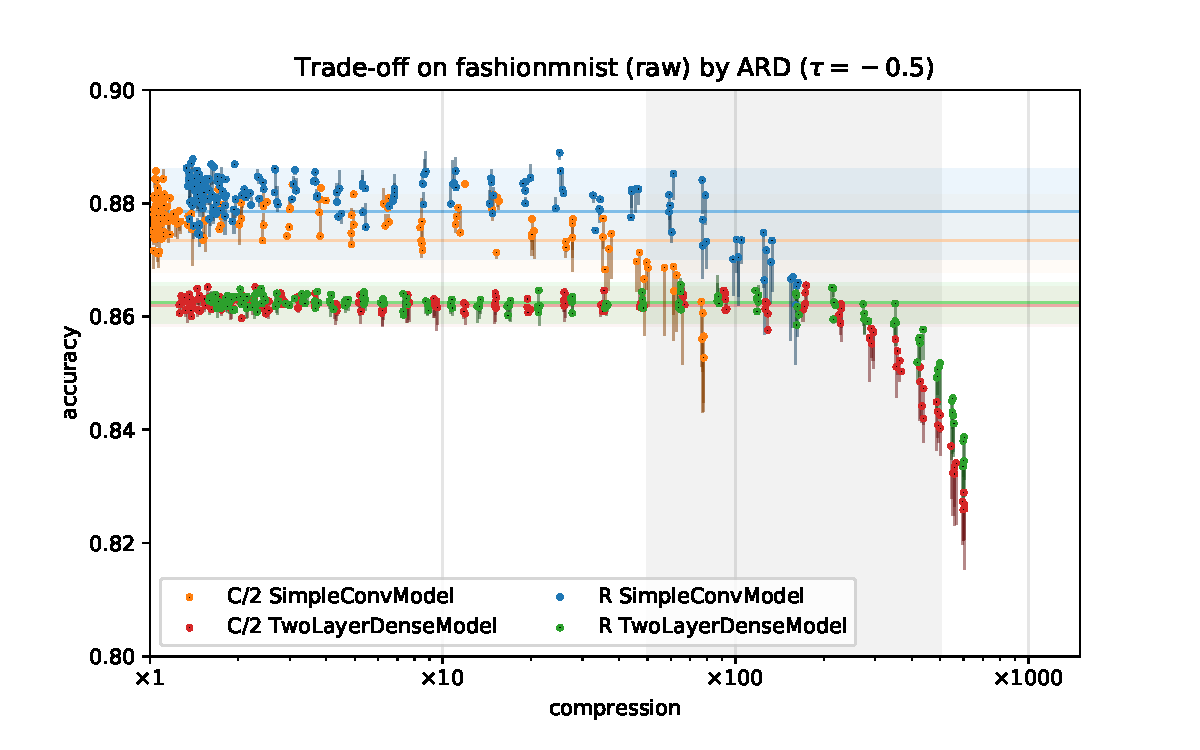
\includegraphics[width=\linewidth]{figure__mnist-like__trade-off/appendix__cmp__ARD__fashionmnist__raw__-0.5.pdf}
  \end{subfigure}%
  \begin{subfigure}[b]{0.5\textwidth}
    \centering
    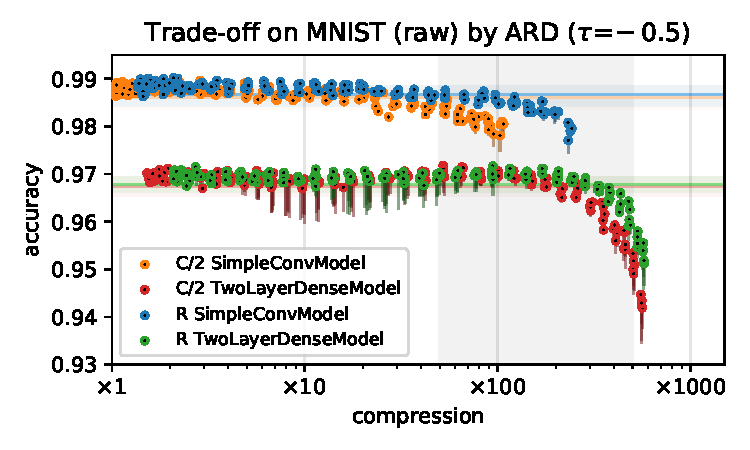
\includegraphics[width=\linewidth]{figure__mnist-like__trade-off/appendix__cmp__ARD__mnist__raw__-0.5.pdf}
  \end{subfigure}
  \caption{%
    The compression-accuracy trade-off of ARD method for $\real$ and $\tfrac12\cplx$ models using raw features.
  }
  \label{fig:appendix__cmp__mnist-like__trade-off__ARD__raw}
\end{figure}

\begin{figure}[ht]
  \centering
  \begin{subfigure}[b]{0.5\textwidth}
    \centering
    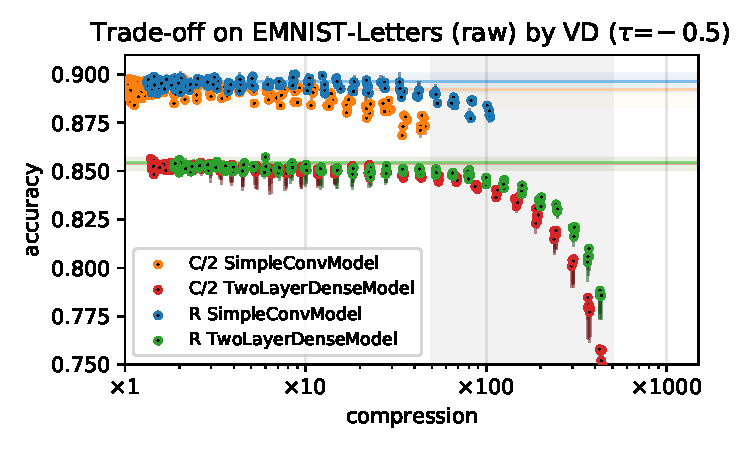
\includegraphics[width=\linewidth]{figure__mnist-like__trade-off/appendix__cmp__VD__emnist_letters__raw__-0.5.pdf}
  \end{subfigure}%
  \begin{subfigure}[b]{0.5\textwidth}
    \centering
    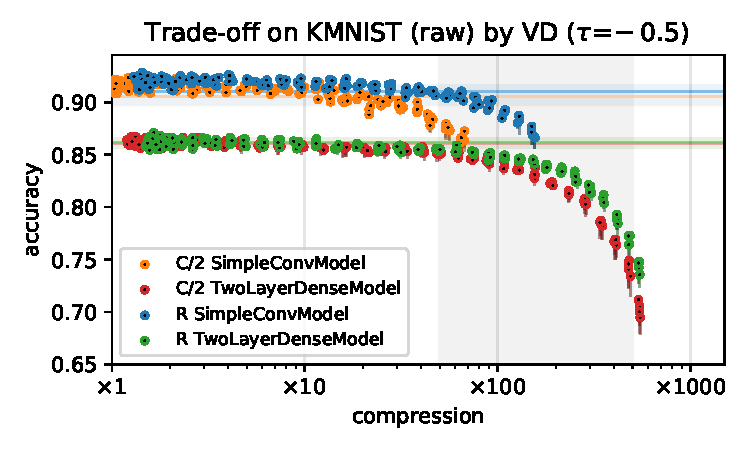
\includegraphics[width=\linewidth]{figure__mnist-like__trade-off/appendix__cmp__VD__kmnist__raw__-0.5.pdf}
  \end{subfigure} \\%
  \begin{subfigure}[b]{0.5\textwidth}
    \centering
    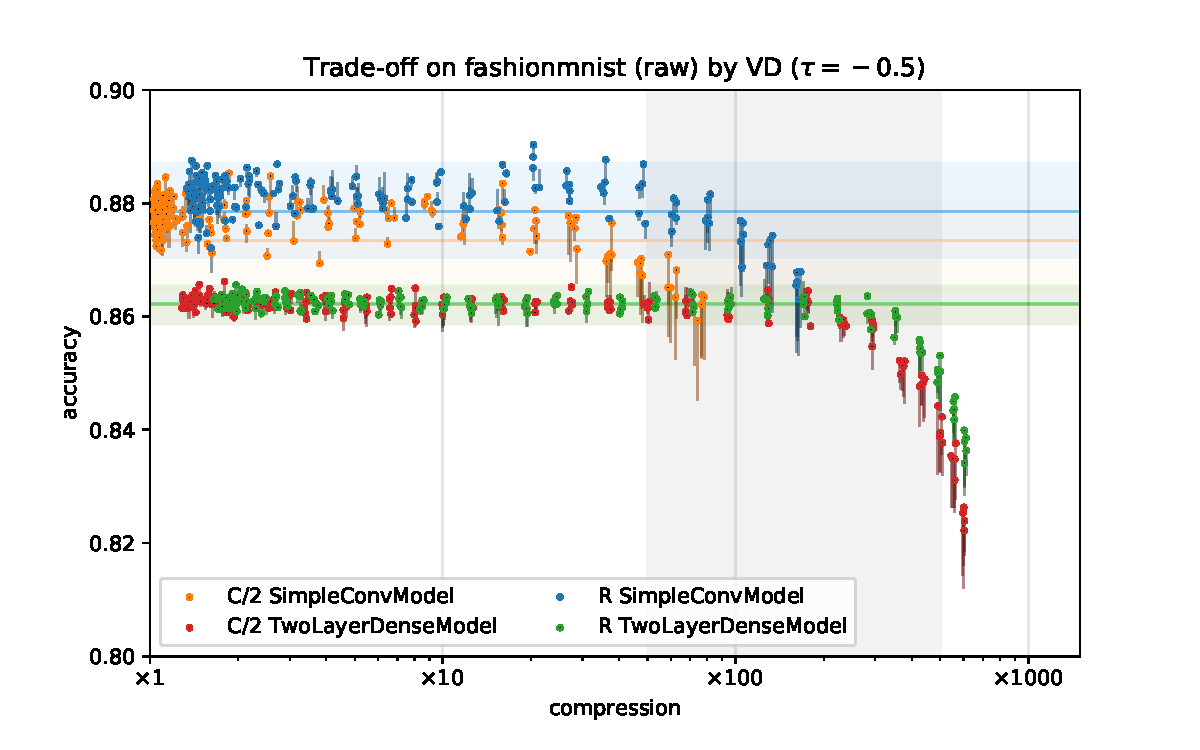
\includegraphics[width=\linewidth]{figure__mnist-like__trade-off/appendix__cmp__VD__fashionmnist__raw__-0.5.pdf}
  \end{subfigure}%
  \begin{subfigure}[b]{0.5\textwidth}
    \centering
    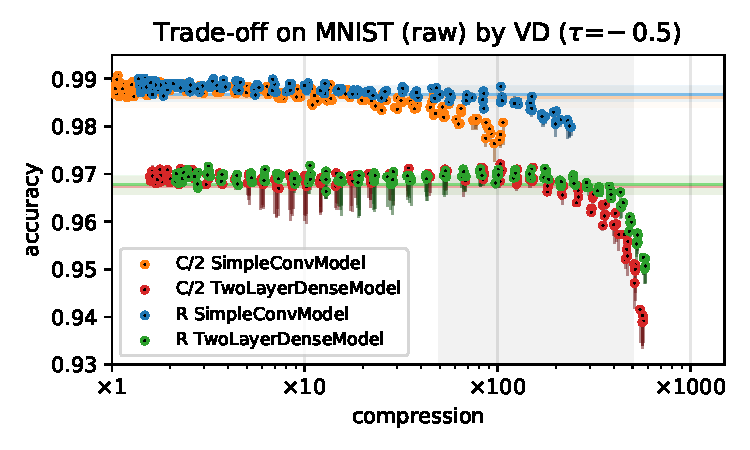
\includegraphics[width=\linewidth]{figure__mnist-like__trade-off/appendix__cmp__VD__mnist__raw__-0.5.pdf}
  \end{subfigure}
  \caption{%
    The compression-accuracy trade-off of VD method for $\real$ and $\tfrac12\cplx$ models using raw features.
  }
  \label{fig:appendix__cmp__mnist-like__trade-off__VD__raw}
\end{figure}

% section mnist_like_experiments (end)

\clearpage

\section{CIFAR10 experiments} % (fold)
\label{sec:cifar_experiments}

For the CIFAR10 experiment we reuse the setup of the MNIST-like experiment with the
following exceptions:
\begin{itemize}
  \item we allocate $20$, $40$, and $20$ epochs to each stage
  \item the weight of the KL divergence term varies over a smaller grid $
    C \in \{
      \tfrac32 2^{-\tfrac{k}2} \colon k=7, \cdots, 15
    \}
  $
  \item we use full $50$k training split of the CIFAR10 dataset for training and raw color
  features only
  \item dataset is randomly augmented: every image within a batch of size $128$ is randomly
  cropped and flipped horizontally
\end{itemize}
Random cropping is done by zero-padding each side of a $32\times 32$ image by four pixels
and then a extracting a random $32\times 32$ patch from the $40\times 40$ intermediate image.

We experiment with $\real$ VGG16 network \citep{simonyan_very_2015} and its $\cplx$-valued
variant, which straightforwardly replaces $\real$ layers with their $\cplx$ counterparts.

\begin{figure}[!ht]
  \centering
  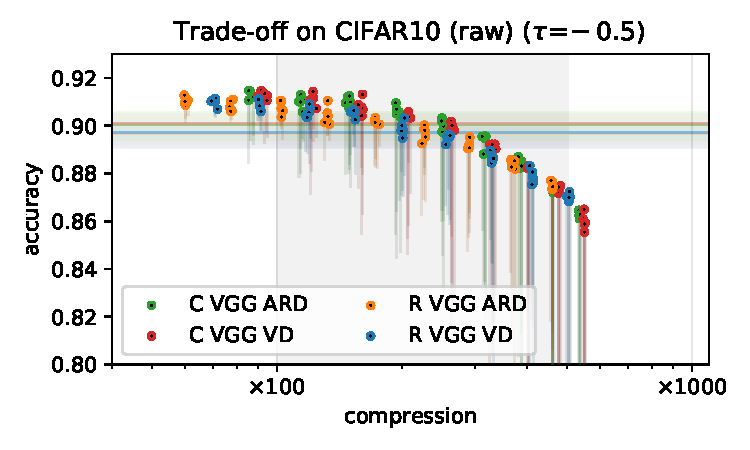
\includegraphics[width=\linewidth]{figure__cifar__trade-off/appendix__augmentedcifar10__raw__-0.5.pdf}
  \caption{%
    The compression-accuracy trade-off for $\real$ and $\cplx$ VGG16 using raw input features.
  }
  \label{fig:appendix__cifar__trade-off__VGG16__raw}
\end{figure}

% section cifar_experiments (end)

\clearpage

\bibliographystyle{abbrvnat}
\bibliography{references}

\end{document}
